\documentclass[preprint]{elsarticle}
\usepackage{float}
\usepackage{amsmath}
\usepackage{amssymb}
\usepackage{csquotes}
\usepackage{longtable}
\usepackage{microtype}

\usepackage{tikz}
\usetikzlibrary{trees, positioning}
\tikzset{
  edge from parent/.style = {draw,
    edge from parent fork right
  },
  basic/.style = {draw,
    align = center,
    font=\fontsize{8}{8}\selectfont
  },
  dots/.style = {
    font=\large
  },
  dots_large/.style = {
    font=\LARGE
  },
  root/.style = {basic},
  level 1/.style = {basic,
    text width = 75pt,
    level distance = 95pt,
    sibling distance = 80pt
  },
  level 2/.style = {basic,
    text width = 110pt,
    level distance = 130pt,
    sibling distance = 42pt
  }
}

\newtheorem{theorem}{Theorem}
\newproof{proof}{Proof}

\DeclareMathOperator{\sign}{sign}

\biboptions{numbers,sort&compress}
\bibliographystyle{elsarticle-num}

\begin{document}

\begin{frontmatter}

\title{Convergence conditions and numerical comparison of global optimization methods based on dimensionality reduction schemes}

% Authors
\author[russia_address]{Vladimir Grishagin\corref{cor_vagris}}
\ead{vagris@unn.ru}

\author[russia_address]{Ruslan Israfilov}
\ead{ruslan@israfilov.com}

\author[russia_address,italy_address]{Yaroslav Sergeyev}
\ead{yaro@dimes.unical.it}

\address[russia_address]{Department of Software and Supercomputing, Lobachevsky State University, Gagarin Avenue 23, 603950 Nizhni Novgorod, Russia.}
\address[italy_address]{DIMES, Università della Calabria, Italy.}

\cortext[cor_vagris]{Corresponding author}

\begin{abstract}
This paper is devoted to numerical global optimization algorithms applying several ideas to reduce the problem dimension. Two approaches to the dimensionality reduction are considered. The first one is based on the nested optimization scheme that reduces the multidimensional problem to a family of one-dimensional subproblems connected in a recursive way. The second approach as a reduction scheme uses Peano-type space-filling curves mapping multidimensional domains onto one-dimensional intervals. In the frameworks of both the approaches, several univariate algorithms belonging to the characteristical class of optimization techniques are used for carrying out the one-dimensional optimization. Theoretical part of the paper contains a substantiation of global convergence for the considered methods. The efficiency of the compared global search methods is evaluated experimentally on the well-known GKLS test class generator used broadly for testing global optimization algorithms. Results for representative problem sets of different dimensions demonstrate a convincing advantage of the adaptive nested optimization scheme with respect to other tested methods.
\end{abstract}

\begin{keyword}
Multiextremal functions, global optimization, numerical methods, dimensionality reduction, convergence, comparison of efficiency.
\MSC[2010] 65K05\sep 90C26
\end{keyword}

\end{frontmatter}

\section{Introduction}
In this paper the black-box global optimization problem
\begin{gather}
  \label{eq:go_problem}
  f^* = f(y^*) = \min_{y \in P} f(y), \\
  \label{eq:hyper}
  P = \{ y \in \mathbb{R}^N \colon a_i \leq y_i \leq b_i, \; 1 \leq i \leq N \},
\end{gather}
%
is considered as a problem of finding the global minimum value $f^*$ and global minimizers $y^* \in P$ of a real-valued multivariate function $f(y)$ in the hyperparallelepiped~(\ref{eq:hyper}) of the Euclidean space $\mathbb{R}^N$. The objective function $f(y)$ is supposed to satisfy in the domain $P$ the Lipschitz condition
\begin{equation}
  \label{eq:lipschitz}
  |f(y') - f(y'')| \leq L\| y' - y'' \|, \; y', y'' \in P,
\end{equation}
%
where $L > 0$ is a finite constant and $\|*\|$ denotes the Euclidean norm in $\mathbb{R}^N$. In general case, these problems are multiextremal and non-smooth.

The global optimization problem under consideration has been drawing attention of many researchers (see, for example, fundamental monographs~\cite{bib1,bib2,bib3,bib4,bib5,bib6}). On the one hand, problems of this kind are very important from the practical point of view because they arise often in scientific and engineering applications (see, for instance,~\cite{bib4,bib7,bib8,bib9,bib10,bib11,bib12,bib13}). On the other hand, Lipschitzian problems~(\ref{eq:go_problem})--(\ref{eq:hyper}) are very interesting for theoretical study because they have a rich variety of properties and, as a consequence, there is no a \enquote{universal} algorithm for solving multiextremal problems. These circumstances generate many fruitful approaches for solving this class of problems. Given approaches are based on ideas of different nature (both stochastic~\cite{bib5,bib6,bib14,bib16,bib17,bib18} and deterministic~\cite{bib19,bib20,bib21,bib22,bib23,bib24,bib25,bib26,bib27,bib28,bib29,bib30,bib46}), but, in any case, numerical methods of searching for the global optimum are proposed within the frameworks of approaches as a tool for getting a solution sought.

As it was discussed in~\cite{bib5}, the global optimum is an integral characteristic of the problem, i.e., in order to make sure that a point $y^* \in P$ is the global minimizer of the problem~(\ref{eq:go_problem})--(\ref{eq:hyper}) it is required to compare the value $f(y^*)$ with values of the objective function at all points of the domain $P$, but not in a vicinity of $y^*$ only. As a result, when minimizing an essentially multiextremal function, a numerical global optimization method has to build a grid (random or regular) in the feasible domain and the number of grid nodes increases exponentially when rising the problem dimension. This peculiarity causes the substantial complexity of multiextremal problems and dimension is a crucial factor influencing significantly the efficiency of global optimization algorithms.

In this situation, approaches to elaboration of computational schemes reducing the dimension are widely used in the multiextremal optimization. Here we consider two approaches in which the initial multidimensional problem~(\ref{eq:go_problem})--(\ref{eq:hyper}) is reduced to one or several univariate subproblems solved by efficient one-dimensional algorithms. The first approach applies \emph{the nested optimization scheme} in its classical version \cite{bib31,bib32,bib33,bib34,bib35,bib36,bib37} and in its generalization --- \emph{the adaptive nested scheme}~\cite{bib38,bib39}. The second approach is based on \emph{Peano space-filling curves} mapping the multidimensional domain~(\ref{eq:hyper}) onto an interval in one-dimensional space $\mathbb{R}^1$~\cite{bib5,bib40,bib41,bib42,bib43,bib44,bib45,bib47}.

The rest of the paper is organized in the following way. Section~\ref{sec:dim_reduction} describes the basic structures of the reduction schemes mentioned above and the univariate characteristical methods of global optimization to be applied within the reduction structures for solving the internal one-dimensional subproblems. Section~\ref{sec:convergence} is devoted to a theoretical substantiation of the convergence for multidimensional methods combining the reduction schemes with characteristical methods of global search and contains both the known and new theoretical results. Section~\ref{sec:num_exp} presents experimental results of efficiency comparison for the methods described in previous sections on representative sets of multiextremal test functions of various dimensions belonging to the popular test class GKLS~\cite{bib48} with a controllable complexity. Finally, Section~\ref{sec:conclusion} contains a brief conclusion.

\section{Schemes of dimensionality reduction}
\label{sec:dim_reduction}

The first approach to dimensionality reduction called the scheme of nested optimization is based on the well-known relation (see, e.g.,~\cite{bib5,bib26,bib31})
\begin{equation}
  \label{eq:nested_eq}
  \min_{y \in P} f(y) = \min_{y_1 \in [a_1, b_1]} \dots \min_{y_N \in [a_N, b_N]} f(y_1, \dots, y_N).
\end{equation}
%
In order to describe the scheme let us define a family of reduced functions as follows:
\begin{gather}
  f^N(y) \equiv f(y), \\
  f^i(y_1, \dots, y_i) = \min_{y_{i + 1} \in [a_{i + 1}, b_{i + 1}]} f^{i + 1} (y_1, \dots, y_i, y_{i + 1}), \; 1 \leq i \leq N - 1.
\end{gather}
%
Then, according to~(\ref{eq:nested_eq}), in order to find the solution to the multidimensional problem~(\ref{eq:go_problem})--(\ref{eq:hyper}) it is sufficient to solve the one-dimensional problem
\begin{equation}
  \label{eq:subproblem_0}
  f(y^*) = \min_{y_1 \in [a_1, b_1]} f^1(y_1).
\end{equation}
%
But in order to evaluate the function $f^1$ at a fixed point $y_1$ it is necessary to solve the one-dimensional problem of the second level
\begin{equation}
  f^1(y_1) = \min_{y_2 \in [a_2, b_2]} f^2(y_1, y_2),
\end{equation}
%
and so on up to the univariate minimization at the $N$-th level the function $f^N(y) = f(y)$ with fixed coordinates $y_1, \dots, y_{N - 1}$.

Thus, instead of the multidimensional problem~(\ref{eq:go_problem})--(\ref{eq:hyper}) one can solve the set of nested one-dimensional subproblems
\begin{equation}
  \label{eq:subproblem_i}
  \min_{y_i \in [a_i, b_i]} f^i(y_1, \dots, y_{i - 1}, y_i), \; 1 \leq i \leq N,
\end{equation}
%
in which the coordinates $y_1, \dots, y_{i - 1}$ have been already determined by the subproblems of preceding levels. The objective functions $f^i(y_1, \dots, y_i)$ of the subproblems~(\ref{eq:subproblem_i}) satisfy the Lipschitz condition for the corresponding argument $y_i$ subject to the assumption~(\ref{eq:lipschitz}) for the function $f(y)$ (see~\cite{bib51}). Therefore, efficient univariate optimization algorithms can be taken for solving these subproblems. Various combinations of such the algorithms with the nested scheme~(\ref{eq:nested_eq}) have been proposed in~\cite{bib5,bib9,bib26,bib33,bib34,bib35}.

The recursive character of generating the subproblems~(\ref{eq:subproblem_i}) during the optimization forms a hierarchical structure of subordination for these subproblems as a tree where the root is the subproblem~(\ref{eq:subproblem_0}) and the leaves are the
subproblems of the $N$-th level. Fig.~\ref{fig:nested_scheme} shows such a structure for $N = 3$.

Algorithmic implementation of the nested optimization scheme has some features. In the classical version (see, e.g.,~\cite{bib5,bib31}) during solving the root problem~(\ref{eq:subproblem_0}) a new evaluation of the function $f^1$ at a new point (new search iteration), i.e., solving a new subproblem of minimization of $f^2$ at the second level is supposed to be carried out only after the completion of the current iteration. It means that only one minimization subproblem at the second level can be active (can be in the course of solving) because the other subproblems of this level either have been already completed or will be initiated later. Analogously, the same situation takes place at all the rest of levels and at every moment of the multidimensional optimization not more than $N$ univariate subproblems are active and they belong to a path from the root to a leaf. In Fig.~\ref{fig:nested_scheme} one of the possible paths consists of subproblems marked with grey colour. Such organization of computations signifies that the information on the subproblems which have been already completed at the level $i$ is not used during current minimization of a function $f^i$ from~(\ref{eq:subproblem_i}). For example, in Fig.~\ref{fig:nested_scheme} all the subproblems located above the active ones (marked with grey) have been already solved and information on the objective function obtained in the course of solving these subproblems is not used in the currently solved subtasks. Such loss of information leads to increasing the number of trials (evaluations of the objective functions) and worsens the efficiency of optimization. Indeed, if during the minimization of a function $f^i$ from~(\ref{eq:subproblem_i}) we get values higher than ones obtained in a subproblem of the same level solved earlier, then, may be, it is reasonable not to continue solving the current subproblem up to the end and not to spend excessive trials.

This idea is realized \emph{in the adaptive nested optimization scheme} proposed in the paper~\cite{bib38} containing a detailed algorithmic description of the adaptive scheme. The main suggestion is to give up the principle of strict subordination inherent to the classical nested scheme and to use a \emph{simultaneous consideration} of all the univariate subproblems arising in the course of multidimensional optimization. In the adaptive scheme all the generated subproblems are active and a numerical \enquote{measure of quality} for each subproblem is introduced (this measure is called the \emph{subproblem characteristic}). An iteration of the multidimensional optimization consists in the choice of the subproblem with maximal characteristic and carrying out a new trial within this subproblem. Such the approach allows choosing the subproblems with lower values of objective univariate functions~(\ref{eq:subproblem_i}) more often than with the higher ones. The way of defining the subproblem characteristics can be different, but in the case when the univariate characteristical algorithms~\cite{bib49,bib50} are used for solving the subproblems~(\ref{eq:subproblem_i}) (see the general description of these algorithms below) the maximal interval characteristic generating by the algorithm in the course of optimization can be taken as the subproblem characteristic.

The second approach is based on the known fact that a finite interval $[a, b]$ of the real axis and the $N$-dimensional hyperparallelepiped~(\ref{eq:hyper}) are equipollent sets and there exist mappings called \emph{Peano space-filling curves} (or \emph{evolvents}) which map the unit interval $[a, b]$ onto the hyperparallelepiped~(\ref{eq:hyper}) continuously and unambiguously.

Let $y(x)$ be such an evolvent. Let us consider the function
\begin{equation}
  \label{eq:peano_map}
  \varphi(x) = f(y(x))
\end{equation}
%
and the one-dimensional problem
\begin{equation}
  \label{eq:peano_min}
  \varphi^* = \varphi(x^*) = \min_{x \in [a, b]} \varphi(x).
\end{equation}
%
Owing to~(\ref{eq:lipschitz}) the function $f(y)$ is continuous and, because of continuity of $f(y)$ and $y(x)$,
\begin{equation}
  \label{eq:peano_min_2}
  \min_{y \in P} f(y) = \min_{x \in [a, b]} \varphi(x),
\end{equation}
%
and the point $y^* = y(x^*)$ is the global minimizer of the multidimensional problem~(\ref{eq:go_problem})--(\ref{eq:hyper}).

As a result, solving the univariate problem~(\ref{eq:peano_min}) allows obtaining the solution to the initial problem~(\ref{eq:go_problem})--(\ref{eq:hyper}). A wide spectrum of the methods exploiting this idea is presented, for example, in publications~\cite{bib5,bib29,bib40,bib43,bib44,bib45,bib47}. It should be noticed that the objective function $\varphi(x) = f(y(x))$ of the univariate problem~(\ref{eq:peano_min}) satisfies in general case the H\"older condition
\begin{equation}
  \label{eq:holder}
  | \varphi(x') - \varphi(x'') | \leq H \sqrt[N]{|x' - x''|}, \; x', x'' \in [a, b],
\end{equation}
%
if the function $f(y)$ is Lipschitzian~(\ref{eq:lipschitz}), and the resulting H\"older constant $H$ is finite and depends on the Lipschitz
constant $L$ and the dimension $N$~\cite{bib5,bib51} only.


Combinations of the reduction schemes described above with different univariate techniques of global search generate corresponding multidimensional algorithms of solving the multiextremal problem~(\ref{eq:go_problem})--(\ref{eq:hyper}). Since in the nested optimization schemes (both classical and adaptive) all the univariate subproblems~(\ref{eq:subproblem_i}) satisfy the Lipschitz condition, we considered as one-dimensional methods the known algorithms of Lipschitzian optimization proposed by Piyavskij~\cite{bib26} and Strongin~\cite{bib15} which are theoretically substantiated and quite efficient. In regard to the reduction on the base Peano evolvents, the reduced objective function~(\ref{eq:peano_map}) is H\"olderian (\ref{eq:holder}) and for solving the univariate problem (\ref{eq:peano_min_2}) it is necessary to apply the methods oriented at this class of optimization problems. As such the methods we took two algorithms which are generalizations~\cite{bib5,bib29} of the Piyavskij's and Strongin's methods mentioned above.

All the univariate methods chosen for our research belong to the class of characteristical algorithms introduced by Grishagin~\cite{bib50} (see also~\cite{bib49}). Therefore, at first we describe a general structure of the characteristical methods and then give in details the specificity of each method in the framework of the general description.

Let us consider the problem of univariate optimization in a standardized form: to find the minimal value
\begin{equation}
  \label{eq:univariate}
  \varphi^* = \varphi(x^*) = \min_{x \in [a, b]} \varphi(x)
\end{equation}
%
of a function $\varphi(x)$ over a finite interval $[a, b] \subset \mathbb{R}^1$ where the objective function $\varphi(x)$ satisfies either Lipschitz~(\ref{eq:lipschitz}) or H\"older~(\ref{eq:holder}) condition in the feasible domain $[a,b]$.

Let the term \enquote{trial} denote an operation that calculates the value of the function $\varphi(x)$ at a point $x \in [a, b]$. An optimization method is supposed to place sequentially trials at points $x^1, x^2, \dots, x^k, \dots $ with corresponding outcomes $z^k = \varphi(x^k)$, $k = 1, 2, \dots$.

A numerical method of solving the problem~(\ref{eq:univariate}) is characteristical if its decision rule of planning trials consists of the following actions.

The first two trials are to be carried out at the end-points of the interval $[a, b]$, i.e.,
\begin{equation}
  x^1 = a, \; x^2 = b,
\end{equation}
with the values $z^1 = \varphi(a)$, $z^2 = \varphi(b)$.

The point $x^{k + 1}$, $k > 2$, of any subsequent $(k + 1)$-th trial is chosen in accordance with the following steps:
\begin{enumerate}[Step 1.]
  % Change spacing between items due to text blending
  \setlength\itemsep{0.5em}

  \item All the points $x^1, x^2, \dots, x^k$ of preceding trials are renumbered by subscripts in increasing order, i.e.,
  \begin{equation}
    \label{eq:x_sorted}
    a = x_1 < x_2 < \dots < x_k = b.
  \end{equation}
  %
  The values $z_i = \varphi(x_i)$, $1 \leq i \leq k$, are juxtaposed to the points $x_i$, $1 \leq i \leq k$, from~(\ref{eq:x_sorted}).

  \item For each subinterval $(x_{i - 1}, x_i)$, $2 \leq i \leq k$, a numerical value $R(i)$ is calculated (this value is called characteristic of the subinterval).

  \item The subinterval $(x_{t - 1}, x_t)$ with the maximal characteristic is selected among all the subintervals:
  \begin{equation}
    \label{eq:r_max}
    R(t) = \max_{2 \leq i \leq k} R(i).
  \end{equation}

  \item The next $(k + 1)$-th trial is executed at a point $x^{k + 1} \in (x_{t - 1}, x_t)$ and the value $z^{k + 1} = \varphi(x^{k + 1})$ is calculated.
\end{enumerate}

The general conditions of convergence to global minimum for characteristical algorithms have been proven in~\cite{bib49}. In particular, these results substantiate the termination criterion in the form
\begin{equation}
  \label{eq:stop_criterion}
  x_t - x_{t - 1} \leq \varepsilon,
\end{equation}
%
where $t$ is the argument of the largest characteristic $R(t)$ from~(\ref{eq:r_max}) and $\varepsilon > 0$ is a predefined coordinate accuracy of the search, i.e., rules 1--4 are carried out until the length of the interval with maximal characteristic is
less than the accuracy $\varepsilon$.

Now in order to describe a characteristical algorithm it is sufficient to define the expressions for its characteristics and the rule of placement of the next trial within the interval with maximal characteristic.

Following this way, we give corresponding descriptions for 4 univariate characteristical methods used in the reduction schemes under consideration.

The first two methods are intended for optimization of univariate Lipschitzian functions and are used in classical and adaptive nested schemes.

The first method was proposed by Piyavskij~\cite{bib26} and it is well-known in the Lipschitzian optimization. Its characteristics $R(i)$ are calculated as
\begin{equation}
  R(i) = \frac{m (x_i - x_{i - 1})}{2} - \frac{z_{i - i} + z_i}{2},
\end{equation}
%
and the point of new trial is calculated in accordance with the expression
\begin{equation}
  \label{eq:new_trial}
  x^{k + 1} = \frac{x_{t - 1} + x_t}{2} - \frac{z_t - z_{t - 1}}{2m},
\end{equation}
%
where $m > 0$ is the parameter of the method. We will use for short designation of this algorithm the abbreviation
PM (\emph{Piyavskij's Method}).

The second algorithm was proposed by Strongin~\cite{bib5,bib15,bib51}. It has the characteristics
\begin{equation}
  R(i) = m (x_i - x_{i - 1}) + \frac{(z_i - z_{i - 1})^2}{m (x_i - x_{i - 1})} - 2 (z_{i - 1} + z_i),
\end{equation}
%
and its new trial point $x^{k + 1}$ is given in accordance with the relation~(\ref{eq:new_trial}). The value $m > 0$ is the parameter of the method. The author of the method called it simply \emph{Global Search Algorithm} and we keep this name in the short form GSA.

If the objective function in the problem~(\ref{eq:univariate}) satisfies the Lipschitz condition with the Lipchitz constant $L > 0$ then the convergence to all global minima is provided by the methods described when the parameter $m > L$ for PM and $m > 2L$ in GSA. Unfortunately, the value of the Lipchitz constant is unknown, as a rule, and for the parameter $m$ one can use its adaptive estimation~\cite{bib5,bib51}.
\begin{equation}
  \label{eq:m}
  m =
  \begin{cases}
    rM, & M > 0, \\
    1,  & M = 0,
  \end{cases}
\end{equation}
%
where
\begin{equation}
  \label{eq:M}
  M = \max_{2 \leq i \leq k} \frac{|z_i - z_{i - 1}|}{x_i - x_{i - 1}}
\end{equation}
%
and $r > 1$ is the parameter of the method.

The next two algorithms are oriented at solving the problem~(\ref{eq:peano_min_2}) with a H\"olderian objective function and are generalizations of PM and GSA to this case. The third methods called GPM (Generalized Piyavskij's Method) uses the characteristics
\begin{equation}
  R(i) = \frac{m \sqrt[N]{x_i - x_{i - 1}}}{2} - \frac{z_{i - 1} + z_i}{2},
\end{equation}
%
and the new trial point
\begin{equation}
  \label{eq:general_new_trial}
  x^{k + 1} = \frac{x_{t - 1} + x_t}{2} - \sign(z_t - z_{t - 1}) \frac{|z_t - z_{t - 1}|^N}{2 r m^N}.
\end{equation}

The fourth method --- Generalized Global Search Algorithm (GGSA) contains the characteristics
\begin{equation}
  R(i) = m \sqrt[N]{x_i - x_{i - 1}} + \frac{(z_i - z_{i - 1})^2}{m \sqrt[N]{x_i - x_{i - 1}}} - 2 (z_{i - 1} + z_i),
\end{equation}
%
and the point of the new trial is calculated in accordance with~(\ref{eq:general_new_trial}).

In both the methods the parameter $m$ is taken in the form~(\ref{eq:m}), but instead of~(\ref{eq:M}) the relation
\begin{equation}
  M = \max_{2 \leq i \leq k} \frac{|z_i - z_{i - 1}|}{\sqrt[N]{x_i - x_{i - 1}}},
\end{equation}
%
is used.

\section{Convergence of multidimensional reduction algorithms}
\label{sec:convergence}
Combinations of the nested dimensionality reduction schemes with the univariate methods PM and GSA generate the multidimensional algorithms for solving the problem~(\ref{eq:go_problem}). Let us call these algorithms in the following manner: PM-C and GSA-C are the classical nested scheme with the methods PM and GSA correspondingly at the univariate levels of reduction~(\ref{eq:subproblem_i}), and PM-A and GSA-A realize the adaptive nested scheme in which for the univariate optimizations~(\ref{eq:subproblem_i}) the methods PM and GSA are used respectively.

Convergence to the global solution of the problem~(\ref{eq:go_problem}) was proven for GSA-C in the monograph~\cite{bib51} and for GSA-A in the paper~\cite{bib38}. Moreover, the methods GPM and GGSA provide the property of global convergence as well (see~\cite{bib29,bib51}). As for PM-C and PM-A, the problem of their convergence to absolute minimum was open so far, and in the present paper we give a theoretical substantiation of this important property.

First of all, we prove an auxiliary assertion on the sensitivity of PM to the possible errors in calculations of objective function values.

Describing the general structure of the characteristical algorithms we supposed that the results $z^k$ at the trial points coincide with strict values of the objective function~(\ref{eq:univariate}), i.e., $z^k = \varphi(x^k)$, $k = 0, 1, \dots$. But in the real optimization there are disturbances caused by computational errors. Assume that these errors are bounded by a real number $\xi > 0$. Then~\cite{bib51} the results $z^k$ of trials can be treated as precise values of a function $\omega(x)$ such that
\begin{equation}
  \label{eq:convergence_cond}
  | \omega(x) - \varphi(x) | \leq \xi, \; x \in [a, b].
\end{equation}

After termination of the search caused by the stopping criterion~(\ref{eq:stop_criterion}) the value
\begin{equation}
  \omega_k^* = \min_{1 \leq i \leq k} z^i
\end{equation}
%
may be considered as an approximation of the global minimum $\varphi^*$ of the function $\varphi(x)$ from~(\ref{eq:univariate}). In this case,
the sensitivity of the method to the bounded errors can be estimated by a degree of proximity between $\omega_k^*$ and $\varphi^*$. The next theorem provides such an estimation for the algorithm PM.

\begin{theorem}
  \label{thm:theorem1}
  Assume that after a termination of the search according to the stopping criterion~(\ref{eq:stop_criterion}) there is a truncated sequence of trials $x^1, x^2 \dots, x^k$ generated by PM during minimizing the approximation $\omega(x)$ of the objective function $\varphi(x),~x\in [a,b]$, satisfying the inequality~(\ref{eq:convergence_cond}), and the function $\varphi(x)$ is Lipschitzian with constant $L > 0$. Then the following inequality holds:
  %
  \begin{equation}
    \label{eq:theorem_1_cond}
    | \omega_k^*  - \varphi^* | \leq \frac{L \varepsilon}{2} + \xi,
  \end{equation}
  if the PM's parameter $m > L$.
\end{theorem}

\begin{proof}
  Let us order the elements of the truncated sequence $x^1, x^2, \dots, x^k$ in accordance with the rule~(\ref{eq:x_sorted}) and introduce the designations $\alpha_i = (z_{i - 1} + z_i) / 2$, $\delta_i = x_i - x_{i - 1}$, $2 \leq i \leq k$, where $z_i = \omega(x_i)$, $1 \leq i \leq k$.

  From the Lipschitz condition for the function $\varphi(x)$
  \begin{equation}
    \varphi(x_i) + \varphi(x_{i - 1}) - L\delta_i \leq 2\varphi^*, \; 2 \leq i \leq k,
  \end{equation}
  %
  and owing to~(\ref{eq:convergence_cond})
  \begin{equation}
    z_i - \varphi(x_i) \leq \xi, \; z_{i - 1} - \varphi(x_{i - 1}) \leq \xi, \; 2 \leq i \leq k,
  \end{equation}
  %
  from where
  \begin{equation}
    \alpha_i - \frac{L \delta_i}{2} \leq \xi + \varphi^*, \; 2 \leq i \leq k,
  \end{equation}
  %
  or
  \begin{equation}
    \label{eq:min_alpha_L_delta}
    \min_{2 \leq i \leq k} \Big( \alpha_i - \frac{L \delta_i}{2} \Big) - \xi \leq \varphi^*.
  \end{equation}
  %
  On the other hand, for the point $x_s$ such that $\omega(x_s) = \omega_k^*$ taking into account~(\ref{eq:convergence_cond}) and the inequality $\varphi(x_s) \geq \varphi^*$ we have
  \begin{equation}
    \label{eq:phi_leq_omega_xi}
    \varphi^* \leq \omega_k^* + \xi.
  \end{equation}
  %
  Let the number $q$, $2 \leq q \leq k$, be such that
  \begin{equation}
    \alpha_q - \frac{L \delta_q}{2} = \min_{2 \leq i \leq k} \Big( \alpha_i - \frac{L \delta_i}{2} \Big).
  \end{equation}
  %
  Let us consider two cases.
  The first one corresponds to the situation $\delta_q \leq \varepsilon$ for $\varepsilon$ from~(\ref{eq:stop_criterion}). Since $\omega_k^* \leq \alpha_q$ then
  \begin{equation}
    \omega_k^* - \frac{L \varepsilon}{2} \leq \alpha_q - \frac{L \delta_q}{2} \leq \alpha_i - \frac{L \delta_i}{2}
  \end{equation}
  %
  for all $i$, $2 \leq i \leq k$.

  In the opposite case $\delta_q > \varepsilon$ let us take the interval $(x_t, x_{t - 1})$ with the largest characteristic $R(t)$ from~(\ref{eq:r_max}) which the inequality~(\ref{eq:stop_criterion}) is true for. The characteristic $R(q) \leq R(t)$ because of~(\ref{eq:r_max}), i.e.,
  \begin{equation}
    R(t) - R(q) = \frac{m(\delta_t - \delta_q)}{2} - \alpha_t + \alpha_q \geq 0,
  \end{equation}
  %
  from where
  \begin{equation}
    \alpha_t - \frac{L \delta_t}{2} \leq \alpha_q - \frac{L \delta_q}{2} - \frac{(m - L)(\delta_q - \delta_t)}{2} \leq \alpha_q -\frac{L \delta_q}{2},
  \end{equation}
  %
  taking into account $m > L$ and $\delta_q > \varepsilon \geq \delta_t$.

  But $\alpha_t - L \delta_t / 2 \geq \omega_k^* - L \varepsilon / 2$, therefore, from~(\ref{eq:min_alpha_L_delta}) it follows that
  \begin{equation}
    \label{eq:omega_phi_leq_frac_xi}
    \omega_k^* - \varphi^* \leq \frac{L \varepsilon}{2} + \xi.
  \end{equation}
  %
  On the other hand, due to~(\ref{eq:phi_leq_omega_xi}) we have
  \begin{equation}
    \label{eq:xi_two_sides}
    \varphi^* - \omega_k^* \leq \xi \leq \xi + \frac{L \varepsilon}{2}.
  \end{equation}
  %
  The inequalities~(\ref{eq:omega_phi_leq_frac_xi}),~(\ref{eq:xi_two_sides}) prove the main assertion~(\ref{eq:theorem_1_cond}) of the theorem. The proof has been completed.
\end{proof}

Now let us return to the multidimensional problem~(\ref{eq:go_problem}) and the algorithm PM-C. It should be noted that the univariate subproblems~(\ref{eq:subproblem_i}) are solved approximately. Indeed, the evaluation of the function $f^{N - 1}(y_1,$ $\dots, y_{N - 1})$ for fixed $y_1, \dots, y_{N - 1}$ consists in minimization by means of PM the function $f^N(y_1,$ $\dots, y_{N - 1}, y_N)$ for the coordinate $y_N$ and instead of the precise value $f^{N - 1}(y_1,$ $\dots, y_{N - 1})$ we obtain an approximate estimation $\omega^{N - 1}(y_1, \dots, y_{N - 1})$. Furthermore, evaluation $f^{N - 2}(y_1,$ $\dots, y_{N - 2})$ for fixed $y_1, \dots, y_{N - 2}$ is implemented as an approximate minimization of the function $\omega^{N - 1}(y_1,$ $\dots, y_{N - 1})$ and the result of this minimization is an approximate estimation $\omega^{N - 2}(y_1,$ $\dots, y_{N - 2})$, etc., up to obtaining an estimation $\omega^* = \omega^1$ in the subproblem $\min \{ \omega^1(y_1) : y_1 \in [a_1, b_1] \}$. In this procedure the resulting value $\omega^*$ is an estimation of the sought solution $f^*$ from~(\ref{eq:go_problem}). As a consequence, in order to ascertain the convergence of PM-C to global minimum of the problem~(\ref{eq:go_problem}) it is sufficient to prove the convergence the estimation $\omega^*$ to $f^*$ when $\varepsilon_1$ (search accuracy in~(\ref{eq:stop_criterion}) for the subproblem~(\ref{eq:subproblem_0})) tends to zero, i.e.,
\begin{equation}
  \label{eq:limit_omega}
  \lim_{\varepsilon_1 \rightarrow 0} \omega^* = f^*.
\end{equation}

If PM is applied for univariate minimization of subproblems~(\ref{eq:subproblem_i}), its parameters can differ at different levels of
recursion, in particular, one can take distinct accuracies in the termination criterion~(\ref{eq:stop_criterion}) and consider the vector
\begin{equation}
  \varepsilon = ( \varepsilon_1, \dots, \varepsilon_N ),
\end{equation}
%
where $\varepsilon_i$ is the termination accuracy during solving the subproblems~(\ref{eq:subproblem_i}) for the coordinate $y_i$, $1 \leq i \leq N$.

\begin{theorem}
  If the objective function $f(y)$ in the problem~(\ref{eq:go_problem}) satisfies the Lipschitz condition~(\ref{eq:lipschitz}) with constant $L > 0$, all the subproblems~(\ref{eq:subproblem_i}) are solved by PM with the parameter $m > L$ and accuracies $\varepsilon_i$ satisfy the inequalities
  \begin{equation}
    \label{eq:eps_next_lower_eps}
    \varepsilon_{i + 1} < \varepsilon_i, \; 1 \leq i < N,
  \end{equation}
  %
  then the assertion~(\ref{eq:limit_omega}) is true.
\end{theorem}

\begin{proof}
  Suppose that for a number $i$, $1 \leq i < N$, the inequality
  \begin{equation}
    \label{eq:f_omega_abs}
    | f^i(y_1, \dots, y_i) - \omega^i(y_1, \dots, y_i) | \leq \xi_i,
  \end{equation}
  %
  holds. This condition is met for $i = N$ with $\xi_N = 0$ as
  \begin{equation}
    \omega^N(y_1, \dots, y_N) = f^N(y_1, \dots, y_N) = f(y).
  \end{equation}

  As the corollary of the Lipschitz condition for the function $f(y)$, all the functions $f^i(y_1, \dots, y_i)$ are Lipschitzian as well with the same constant $L$ (see~\cite{bib51}). Then, in accordance with the Theorem~\ref{thm:theorem1} the inequality~(\ref{eq:f_omega_abs}) involves for the number $i - 1$ the estimation
  \begin{equation}
    | f^{i - 1}(y_1, \dots, y_{i - 1}) - \omega^{i - 1}(y_1, \dots, y_{i - 1}) | \leq \xi_i + \frac{L \varepsilon_i}{2},
  \end{equation}
  %
  and, as consequence, one can take
  \begin{equation}
    \xi_{i - 1} = \xi_i + \frac{L \varepsilon_i}{2}
  \end{equation}
  %
  Since the condition~(\ref{eq:f_omega_abs}) takes place for $i = N$ with $\xi_N = 0$ it is true for all $i$, $1 \leq i \leq N$, and we get the estimation
  \begin{equation}
    \label{eq:phi_omega_diff}
    | \varphi^* - \omega^* | \leq \frac{L}{2} \sum_{i = 1}^N \varepsilon_i,
  \end{equation}

  Then the statement~(\ref{eq:limit_omega}) results immediately from~(\ref{eq:eps_next_lower_eps}) and~(\ref{eq:phi_omega_diff}). The theorem has been proven.
\end{proof}

Finally, for the adaptive nested scheme with the Piyavskij's method inside (PM-A) its convergence follows from the convergence of PM-C by reasons which substantiated in~\cite{bib38} the convergence of GSA-A.

\section{Numerical experiments}
\label{sec:num_exp}
In this section we consider 7 global search algorithms and compare their efficiency experimentally. 6 methods combine the reduction schemes described above with two Lipschitzian one-dimensional methods and their generalizations to the H\"older case and were considered in previous section. To demonstrate the efficiency of these algorithms in comparison with a method of another nature we took the well-known method of Lipschitz optimization DIRECT~\cite{bib23,bib24} as well.

All the methods were compared on the test class of multiextremal functions GKLS from~\cite{bib48} being an easy-to-use source of functions with tuned complexity. The test sets consisting of 100 GKLS problems were taken for each of dimensions 2, 3, 4. For all the dimensions the hard class of GKLS was chosen with the following parameters:
\begin{itemize}
  \setlength\itemsep{0em}

  \item 10 local minima;
  \item radius of the attraction region of the global minimizer equal to $0.12$;
  \item standard function value $-1.0$ at the global minimizer;
  \item distance from the global minimizer to the vertex of the paraboloid equal to $0.9$.
\end{itemize}

The efficiency of algorithms was measured in accordance with the following two criteria: the average number $K$ of trials (evaluations of the objective function) executed during optimization of the functions from the test set and the number $P$ of test problems solved successfully. A test problem was supposed to have been solved if the trial with the lowest value obtained in the course of optimization was placed in a $\delta$-neighbourhood of the global minimizer.

In more details, the values $K$ and $P$ were estimated as follows. The algorithm with a given set of parameters solves $n$ optimization problems from the test class. After solving the $i$-th test problem we have the number $K_i$ of executed trials and the distance
\begin{equation}
  P_i = \sqrt{\sum_{j = 1}^{N} ( y_j^* - y_j^+ )^2}
\end{equation}
%
between the real global minimizer $y^* = (y_1^*, \dots, y_N^*)$ and the coordinate vector $y^+ = (y_1^+, \dots, y_N^+)$ corresponding to the lowest function value found by the algorithm.

After solving all the test problems the criteria $K$ and $P$ are calculated as
\begin{equation}
  K = \frac{1}{n} \sum_{i = 1}^{n} K_i, \quad P = \frac{1}{n}\sum_{i = 1}^{n} p_i,
\end{equation}
%
where for given accuracy $\delta > 0$
\begin{equation}
  p_i =
  \begin{cases}
    1, & P_i <    \delta, \\
    0, & P_i \geq \delta.
  \end{cases}
\end{equation}

Taking these criteria into consideration it is possible to apply the \emph{method of operational characteristics}~\cite{bib39,bib52} which allows one to present comparison results in a visual form. In accordance with this method an optimization algorithm solves problems of a test set several times using different values of its parameters and obtains a pair $(K, P)$ of the efficiency criteria for each variant of parameters chosen. The set of these pairs is called \emph{operational characteristic} of the algorithm. Plotting the operational characteristics on the plane $(K, P)$ enables to compare visually the efficiency of different optimization algorithms. Namely, if for the same $P$ the operational characteristic of an algorithm is located to the left of the characteristic of another method, the first algorithm is better because it has spent less number of trials $K$ for successful solving the same number of problems.

In experiments the algorithms on the base of the reduction schemes used in~(\ref{eq:m}) the identical parameter $r = 8$ providing for all 6 methods the sufficient  conditions of global convergence  and the curves of the operational characteristics for these algorithms and the method DIRECT were obtained by means of variation of parameters in stopping criteria of these methods.

The operational characteristics of the optimization algorithms underwent the examination on the 3-dimensional GKLS set are divided for better visualization into 3 groups and presented in Fig.~\ref{fig:ops_pm},~\ref{fig:ops_gsa},~\ref{fig:ops_gsa_pm}.

Fig.~\ref{fig:ops_pm} and Fig.~\ref{fig:ops_gsa} contain the operational characteristics for the algorithms of PM-type family and for the algorithms of GSA-type family correspondingly. Fig.~\ref{fig:ops_gsa_pm} compares the operational characteristics of the algorithms based on the adaptive nested scheme. In these figures the number of trials is plotted on the abscissa axis in the logarithmic scale.

As it follows from the results presented in Fig.~\ref{fig:ops_pm} and Fig.~\ref{fig:ops_gsa}, among the algorithms combining the methods of the same type with different schemes of dimensionality reduction the adaptive nested scheme is most efficient if it is necessary to solve problems with high reliability $P$. At the same time, the efficiencies of the reduction by means of Peano-type space-filling curves and the classical nested scheme differ slightly. Moreover, all 6 algorithms realizing the dimensionality reduction outperform significantly the method DIRECT.

With regard to comparison of the algorithms having demonstrated the best results in their families, the method GSA-A is some more efficient than PM-A.

The similar conclusions on the efficiency of the compared algorithms can be drawn after the experiments on the 2- and 4-dimensional GKLS classes. As a confirmation Tables~\ref{tab:trials_2d} and~\ref{tab:trials_4d} describe the results of testing for these dimensions. The left column contains the number $K$ of trials and the other columns correspond to the studied methods and show the quantity of problems solved successfully depending on the spent trials.

\section{Conclusion}
\label{sec:conclusion}
Numerical multidimensional global optimization algorithms based on several ideas of a dimensionality reduction have been considered. These algorithms reduce the multidimensional problem to one or several univariate subproblems solved by efficient methods of one-dimensional global optimization. Two approaches to reducing the dimension in multiextremal Lipschitzian optimization problems have been used: the reduction by means of Peano-type space-filling curves and the nested optimization scheme. In the framework of the second approach two versions of the nested reduction have been taken, namely, classical nested scheme and its recent generalization --- adaptive nested optimization. For solving the univariate subproblems the known algorithms proposed by Strongin and Piyavskij and the generalizations of these methods to the class of H\"olderian functions have been used.

For the considered algorithms the theoretical substantiation of convergence to global optimum has been given including both the known results and the new ones proved in the paper. For evaluation of efficiency a representative experimental testing of the methods has been carried out for different dimensions on sets of multiextremal functions belonging to the well-known GKLS test class being at present a classical tool for testing global optimization algorithms. Additionally, the popular method DIRECT has been tested to compare the reduction methods with an algorithm of the other nature. As a result of experiment, among all competitors the adaptive nested scheme has demonstrated the best efficiency.

The promising way of future researches consists in development of parallel algorithms based on the adaptive nested scheme, theoretical investigation of their properties and evaluation of parallelization efficiency, including comparison with existing parallel optimization methods.

\section*{Acknowledgements}
This research was supported by the Russian Science Foundation, project No. 15-11-30022 \enquote{Global optimization, supercomputing computations, and applications}.

\section*{References}
\bibliography{bibliography}

\appendix
\section{}

\begin{figure}[H]
  \centering
  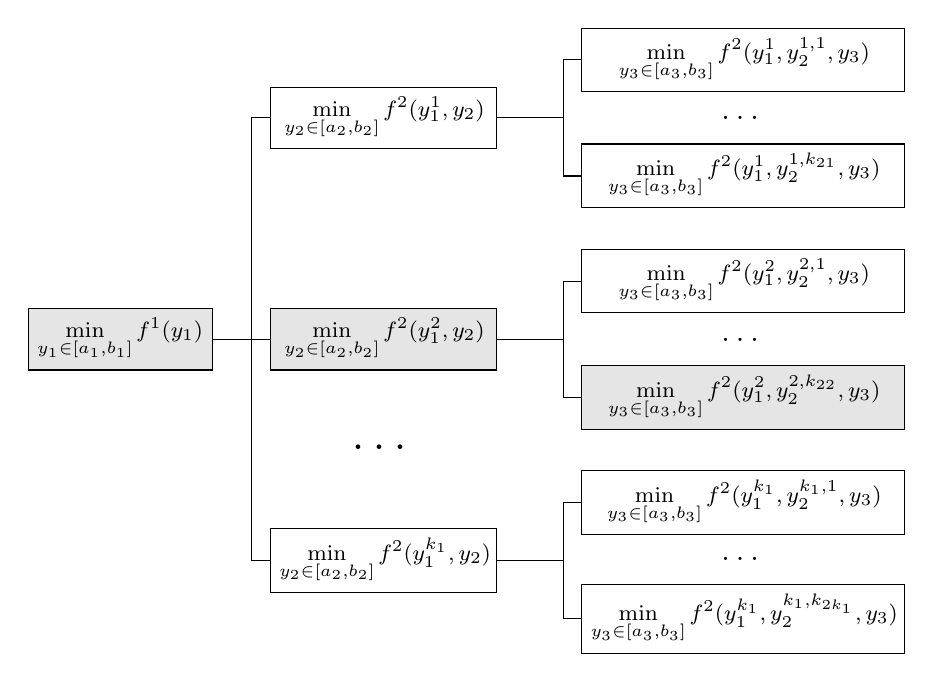
\begin{tikzpicture}
    \node[root, fill = gray!20] {$\displaystyle\min_{y_1 \in [a_1, b_1]} f^1(y_1)$} [grow=right]
      child { node[level 1] (level_1) {$\displaystyle\min_{y_2 \in [a_2, b_2]} f^2(y_1^{k_1}, y_2)$}
        child { node[level 2] (level_2_1) {$\displaystyle\min_{y_3 \in [a_3, b_3]} f^2(y_1^{k_1}, y_2^{k_1, k_{2 k_1}}, y_3)$} }
        child { node[level 2] {$\displaystyle\min_{y_3 \in [a_3, b_3]} f^2(y_1^{k_1}, y_2^{k_1, 1}, y_3)$} }
      }
      child { node[level 1, fill = gray!20] {$\displaystyle\min_{y_2 \in [a_2, b_2]} f^2(y_1^2, y_2)$}
        child { node[level 2, fill = gray!20] (level_2_2) {$\displaystyle\min_{y_3 \in [a_3, b_3]} f^2(y_1^2, y_2^{2, k_{22}}, y_3)$} }
        child { node[level 2] {$\displaystyle\min_{y_3 \in [a_3, b_3]} f^2(y_1^2, y_2^{2, 1}, y_3)$} }
      }
      child { node[level 1] {$\displaystyle\min_{y_2 \in [a_2, b_2]} f^2(y_1^1, y_2)$}
        child { node[level 2] (level_2_3) {$\displaystyle\min_{y_3 \in [a_3, b_3]} f^2(y_1^1, y_2^{1, k_{21}}, y_3)$} }
        child { node[level 2] {$\displaystyle\min_{y_3 \in [a_3, b_3]} f^2(y_1^1, y_2^{1, 1}, y_3)$} }
      };
    \node[dots_large, above = 25pt of level_1] {$\dots$};
    \node[dots, above = 5pt of level_2_1] {$\dots$};
    \node[dots, above = 5pt of level_2_2] {$\dots$};
    \node[dots, above = 5pt of level_2_3] {$\dots$};
  \end{tikzpicture}
  \caption{\label{fig:nested_scheme} The subordination structure of the univariate subproblems~(\ref{eq:subproblem_i})}
\end{figure}

\begin{figure}[H]
  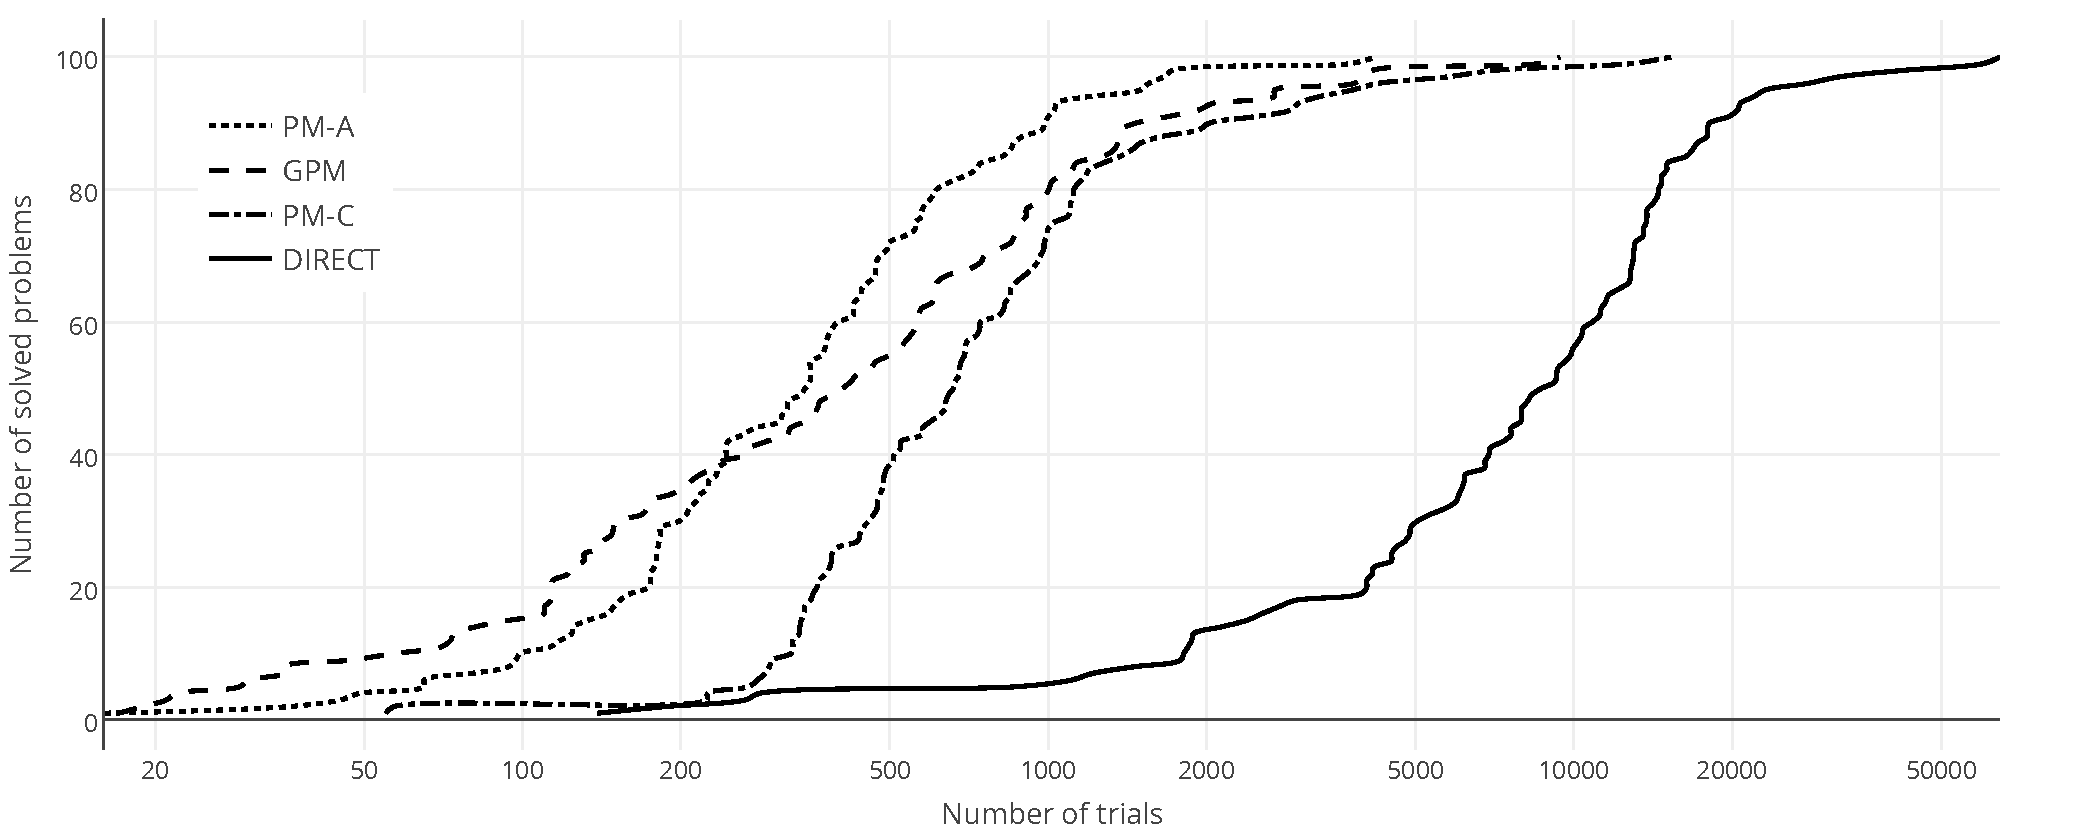
\includegraphics[width=\textwidth]{figure2.pdf}
  \caption{\label{fig:ops_pm} Operational characteristics of PM-type algorithms and DIRECT}
\end{figure}

\begin{figure}[H]
  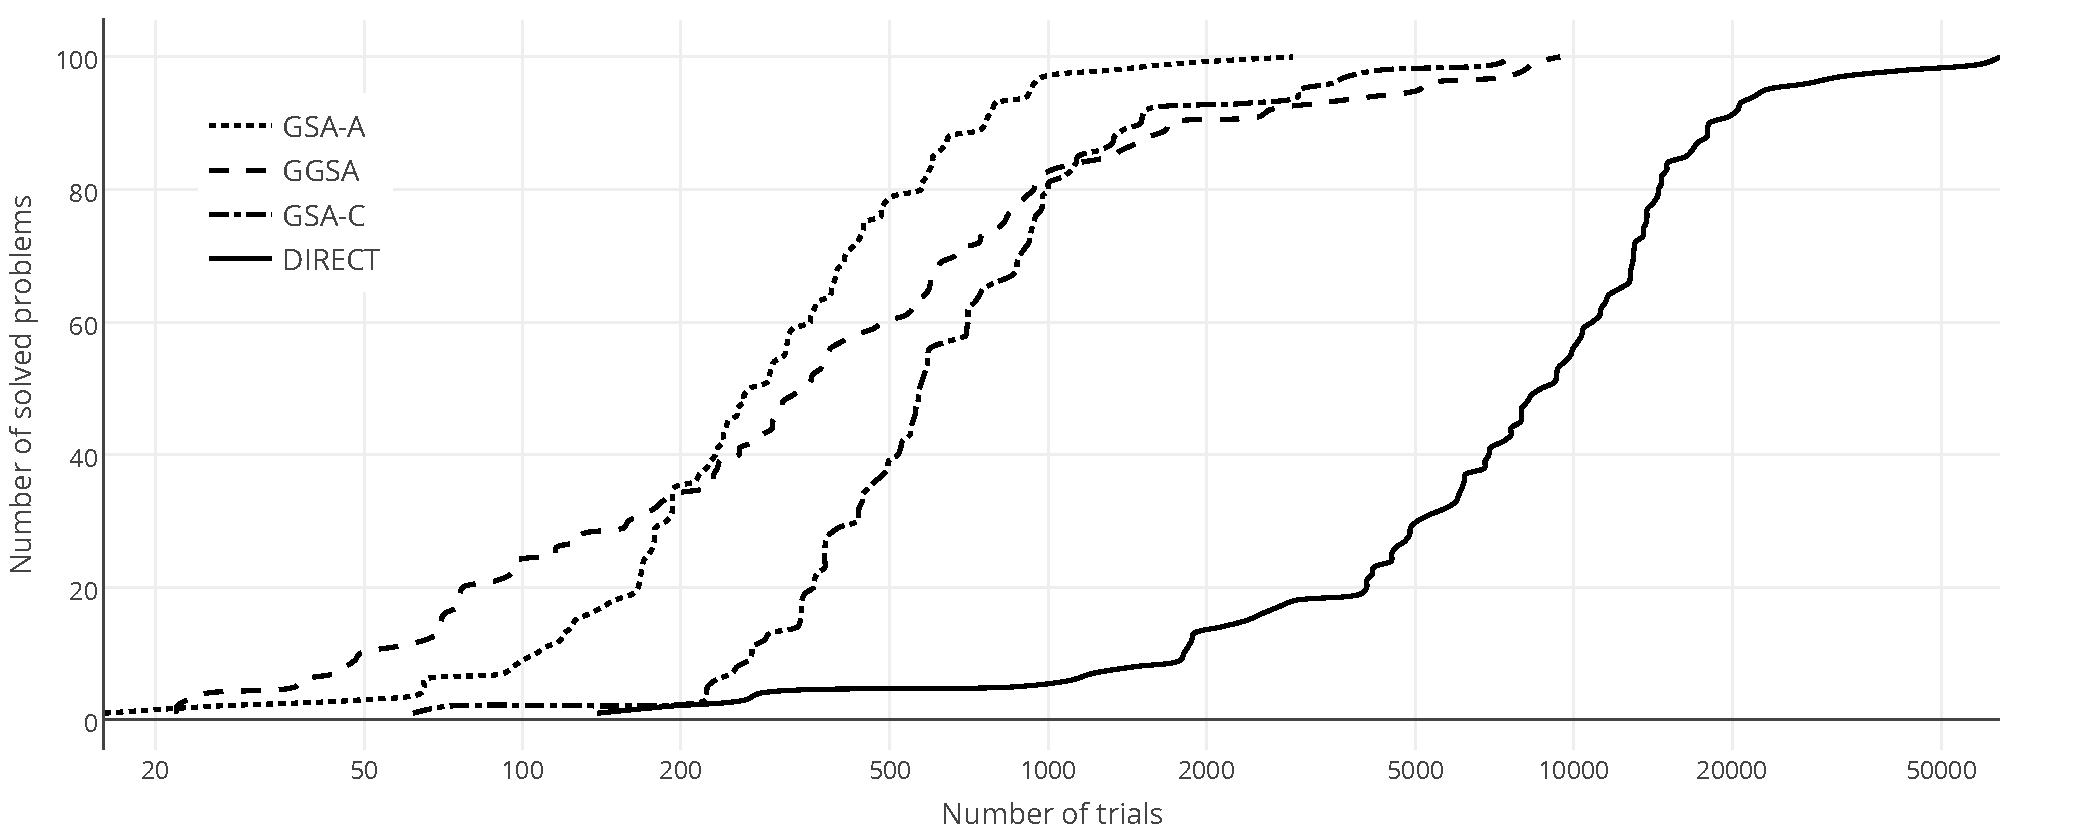
\includegraphics[width=\textwidth]{figure3.pdf}
  \caption{\label{fig:ops_gsa} Operational characteristics of GSA-type algorithms and DIRECT}
\end{figure}

\begin{figure}[H]
  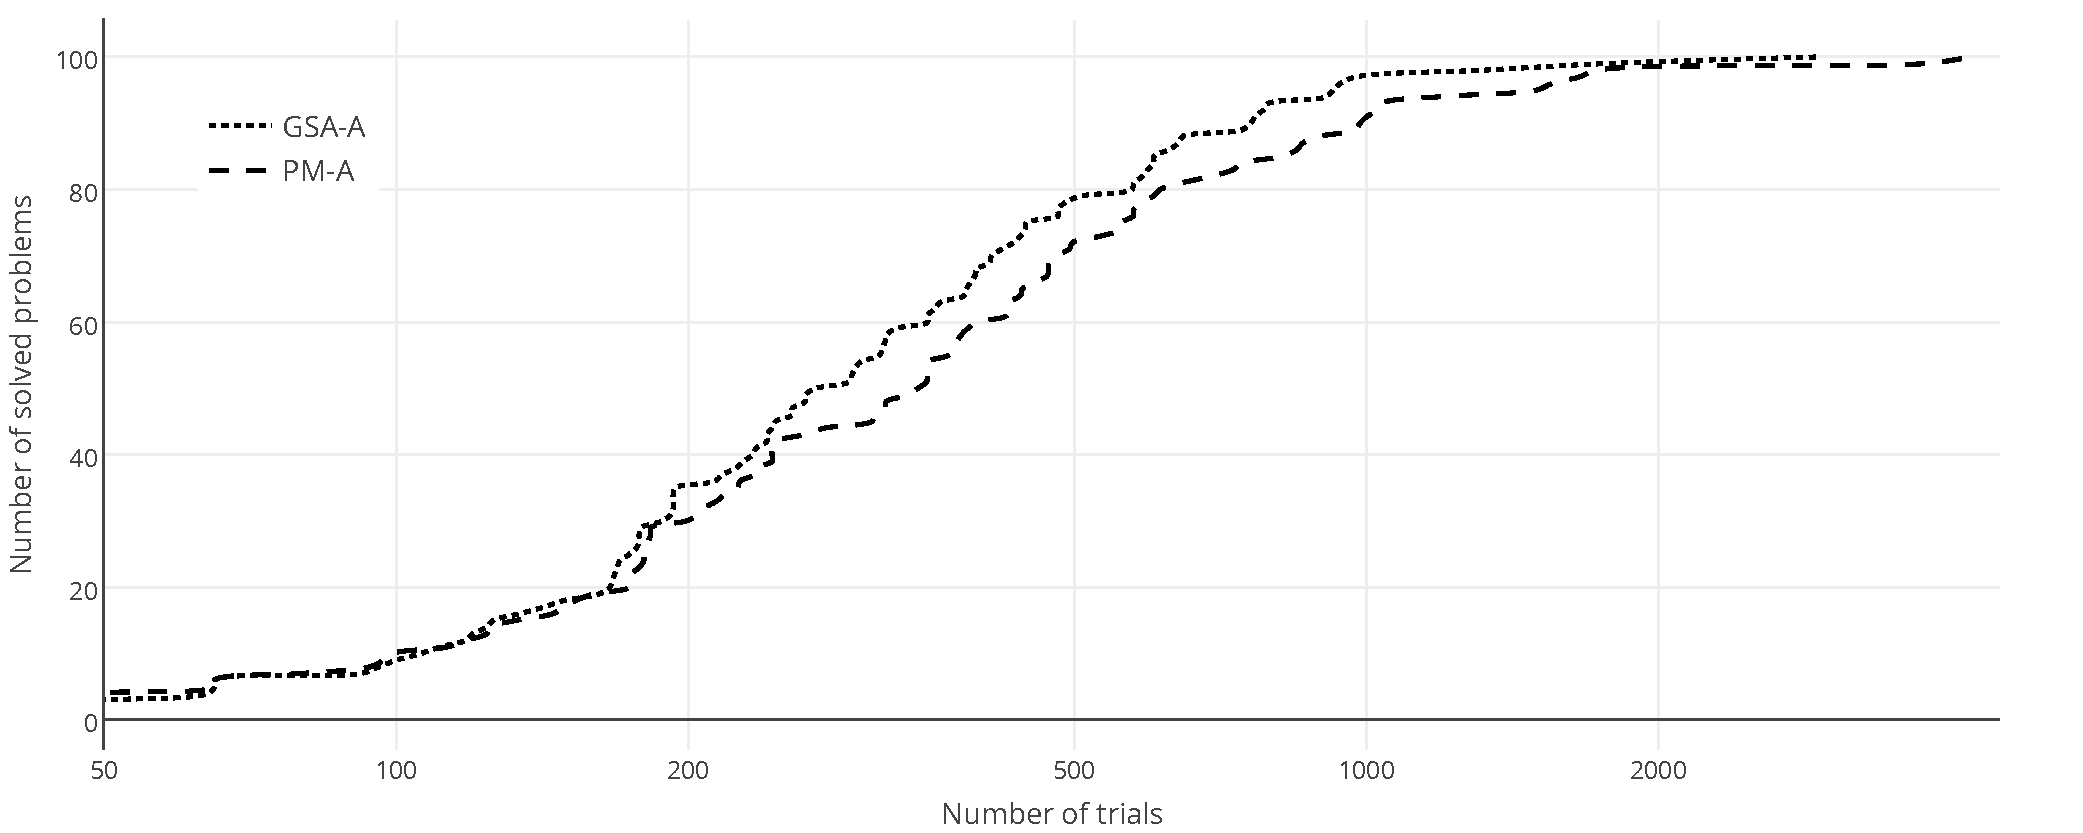
\includegraphics[width=\textwidth]{figure4.pdf}
  \caption{\label{fig:ops_gsa_pm} Operational characteristics of GSA-A and PM-A}
\end{figure}

\begin{center}
  \begin{longtable}{cccccccc}
    \caption{\label{tab:trials_4d} Number of problems solved successfully depending on the executed trials on four-dimensional class} \\
    \hline
    \multicolumn{1}{c}{K}      &
    \multicolumn{1}{c}{GSA-A}  &
    \multicolumn{1}{c}{GSA-C}  &
    \multicolumn{1}{c}{GGSA}   &
    \multicolumn{1}{c}{PM-A}   &
    \multicolumn{1}{c}{PM-C}   &
    \multicolumn{1}{c}{GPM}    &
    \multicolumn{1}{c}{DIRECT} \\
    \hline
    \endfirsthead

    \caption{Number of problems solved successfully depending on the executed trials on four-dimensional class (Continue)} \\
    \hline
    \multicolumn{1}{c}{K}      &
    \multicolumn{1}{c}{GSA-A}  &
    \multicolumn{1}{c}{GSA-C}  &
    \multicolumn{1}{c}{GGSA}   &
    \multicolumn{1}{c}{PM-A}   &
    \multicolumn{1}{c}{PM-C}   &
    \multicolumn{1}{c}{GPM}    &
    \multicolumn{1}{c}{DIRECT} \\
    \hline
    \endhead

    \hline
    \multicolumn{8}{r}{{Continued on the next page}} \\
    \hline
    \endfoot

    \hline
    \endlastfoot

    500    &   6 &   1 &   1 &   1 &   1 &   1 &   1 \\
    1000   &  22 &   1 &  20 &  21 &   1 &  15 &   1 \\
    2000   &  45 &   4 &  34 &  46 &   5 &  29 &   1 \\
    5000   &  82 &  48 &  53 &  79 &  47 &  57 &   1 \\
    10000  &  96 &  78 &  71 &  92 &  72 &  74 &   1 \\
    16000  & 100 &  87 &  79 & 100 &  86 &  83 &   1 \\
    30000  & 100 &  93 &  89 & 100 &  95 &  90 &  20 \\
    50000  & 100 & 100 & 100 & 100 & 100 & 100 &  50 \\
    70000  & 100 & 100 & 100 & 100 & 100 & 100 &  71 \\
    90000  & 100 & 100 & 100 & 100 & 100 & 100 &  81 \\
    120000 & 100 & 100 & 100 & 100 & 100 & 100 & 100 \\
  \end{longtable}
\end{center}

\begin{center}
  \begin{longtable}{cccccccc}
    \caption{\label{tab:trials_2d} Number of problems solved successfully depending on the executed trials on two-dimensional class} \\
    \hline
    \multicolumn{1}{c}{K}      &
    \multicolumn{1}{c}{GSA-A}  &
    \multicolumn{1}{c}{GSA-C}  &
    \multicolumn{1}{c}{GGSA}   &
    \multicolumn{1}{c}{PM-A}   &
    \multicolumn{1}{c}{PM-C}   &
    \multicolumn{1}{c}{GPM}    &
    \multicolumn{1}{c}{DIRECT} \\
    \hline
    \endfirsthead

    \caption{Number of problems solved successfully depending on the executed trials on two-dimensional class (Continue)} \\
    \hline
    \multicolumn{1}{c}{K}      &
    \multicolumn{1}{c}{GSA-A}  &
    \multicolumn{1}{c}{GSA-C}  &
    \multicolumn{1}{c}{GGSA}   &
    \multicolumn{1}{c}{PM-A}   &
    \multicolumn{1}{c}{PM-C}   &
    \multicolumn{1}{c}{GPM}    &
    \multicolumn{1}{c}{DIRECT} \\
    \hline
    \endhead

    \hline
    \multicolumn{8}{r}{{Continued on the next page}} \\
    \hline
    \endfoot

    \hline
    \endlastfoot

    10 &   1 &   1 &   8 &   1 &   1 &  18 &   3 \\
    20 &  35 &  32 &  53 &  30 &  26 &  52 &   6 \\
    30 &  82 &  71 &  80 &  68 &  59 &  71 &   9 \\
    40 &  96 &  94 &  91 &  92 &  86 &  84 &  13 \\
    50 & 100 &  99 &  97 & 100 &  96 &  92 &  16 \\
    80 & 100 & 100 & 100 & 100 & 100 & 100 &  24 \\
   150 & 100 & 100 & 100 & 100 & 100 & 100 &  35 \\
   250 & 100 & 100 & 100 & 100 & 100 & 100 &  47 \\
   500 & 100 & 100 & 100 & 100 & 100 & 100 &  80 \\
   800 & 100 & 100 & 100 & 100 & 100 & 100 & 100 \\
  \end{longtable}
\end{center}

\end{document}
